%
% Chapter 5: MVP/UML Diagrams and Architecture
%
\chapter{System Architecture and UML Diagrams}
\label{chap:architecture}
\setlength{\parskip}{1em}

This chapter describes Snowdrop’s architecture through a set of component diagrams, UML use case and sequence diagrams, and the current design of the Neo4j schema-metadata layer.

\section{System Overview}

Figure~\ref{fig:architecture} shows the overall component architecture of Snowdrop.

\begin{figure}[H]
    \centering
    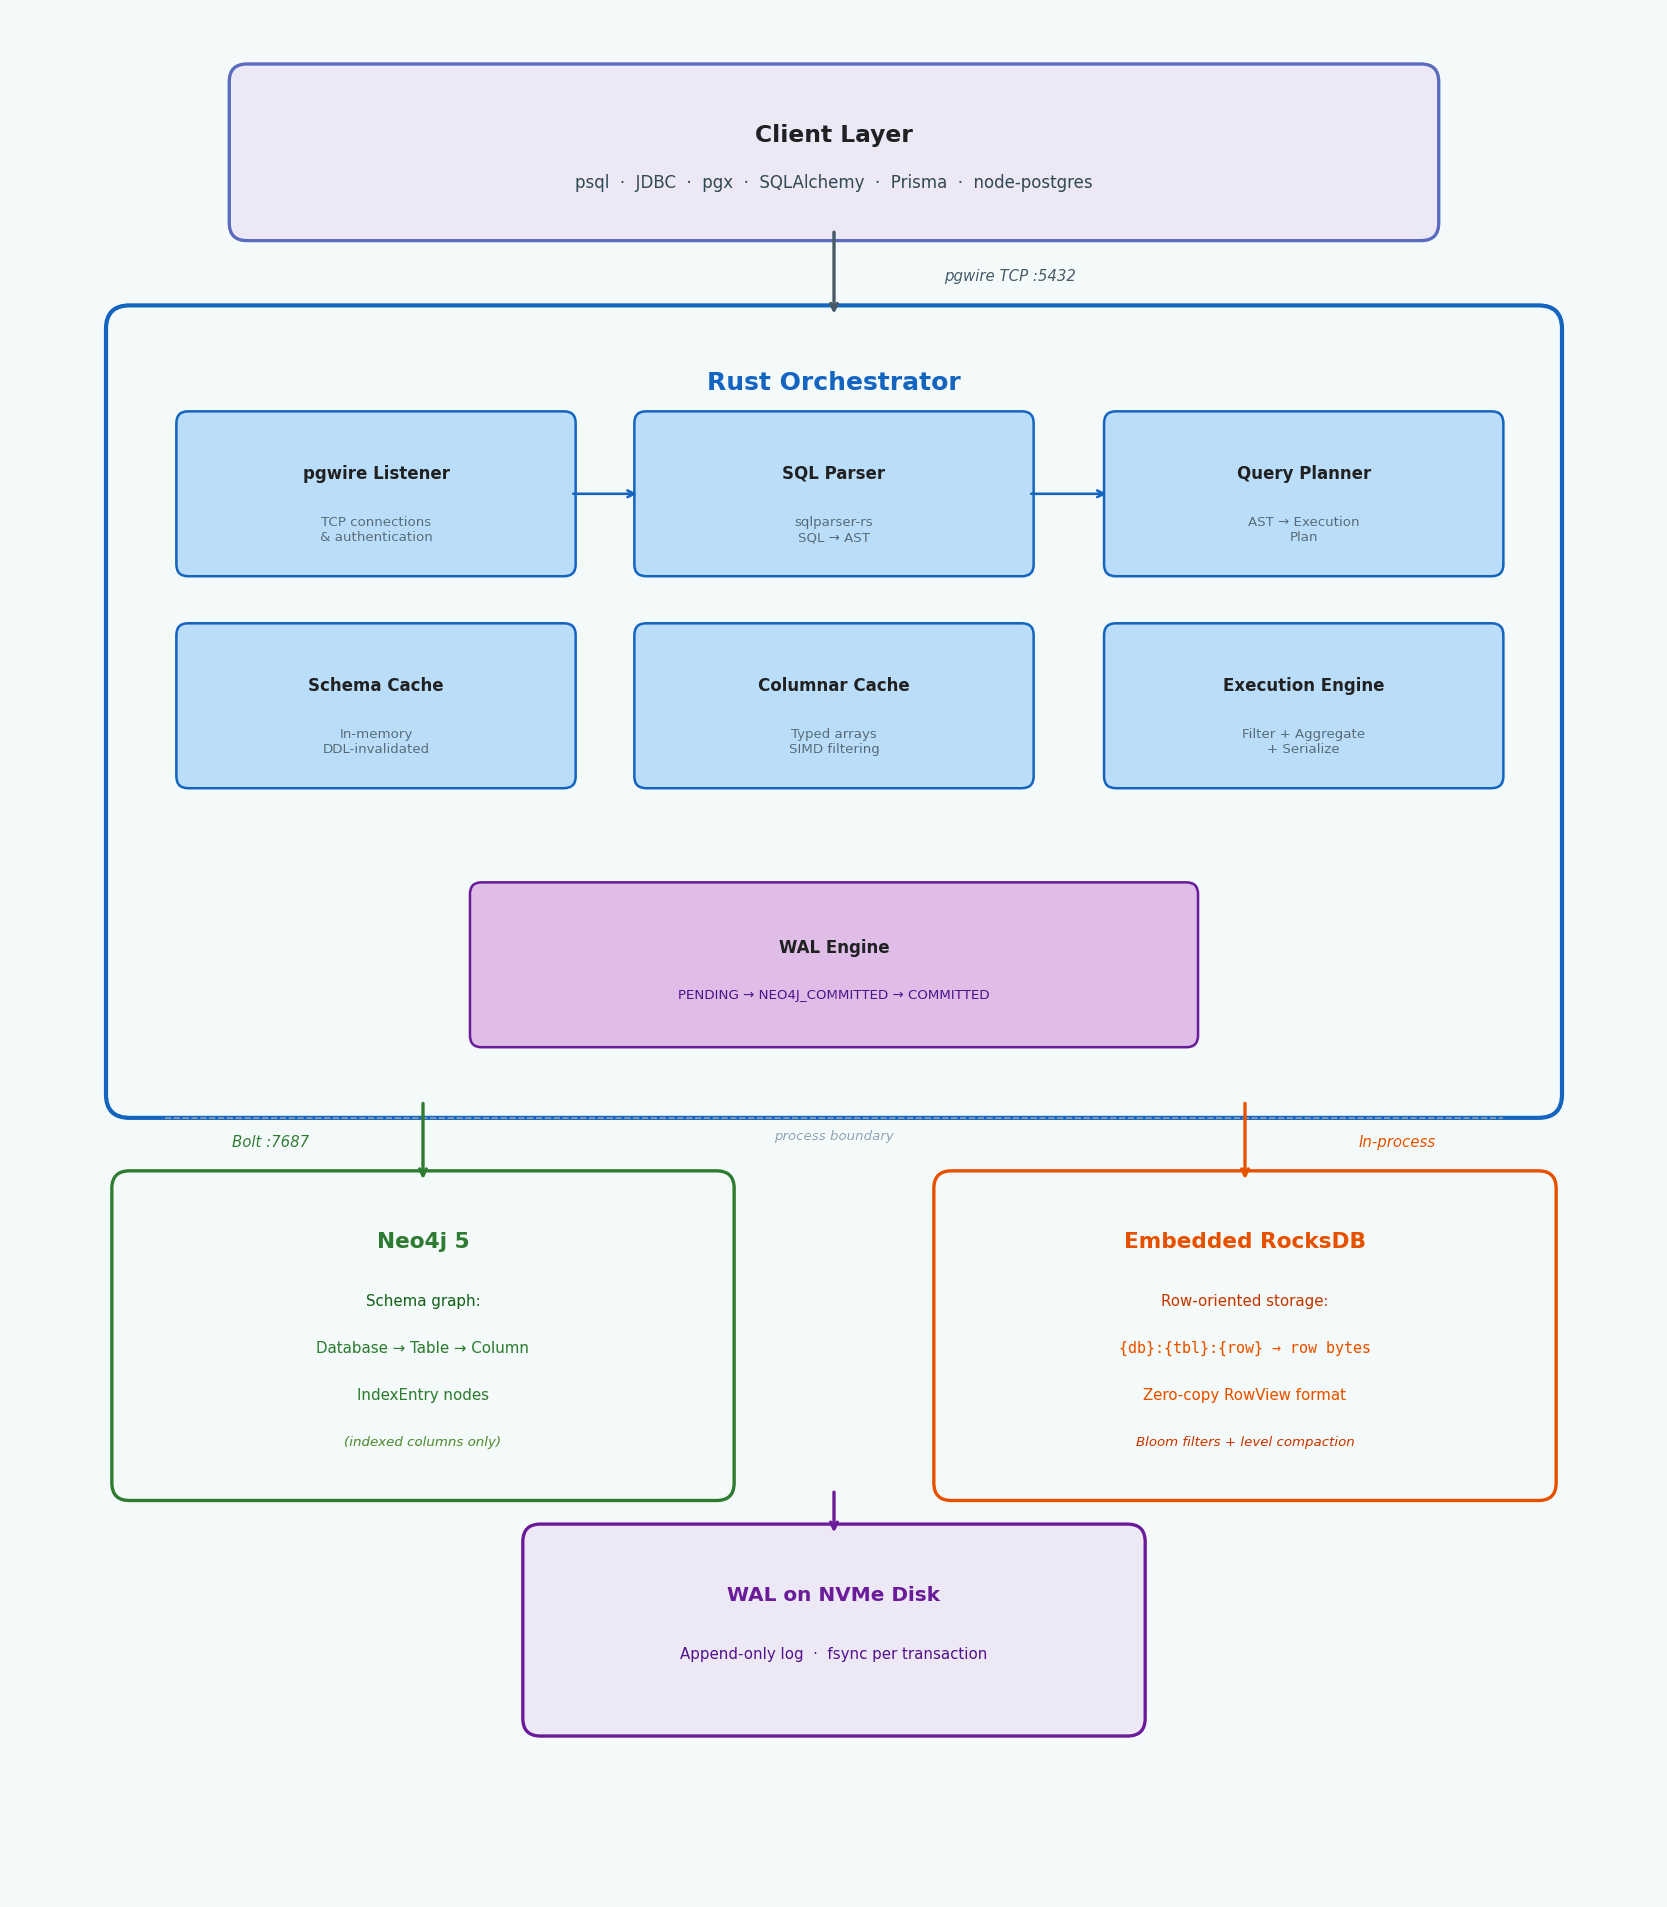
\includegraphics[width=\textwidth]{chapters/chapter05/fig05/01_component_architecture (1).png}
    \caption{Snowdrop component architecture}
    \label{fig:architecture}
\end{figure}

At the center of the system is a Rust-based orchestrator that includes six main subsystems: the pgwire listener, the SQL parser (\texttt{sqlparser-rs}), the query planner, the schema cache, the columnar cache with SIMD-based filtering, and the execution engine. This orchestrator coordinates two storage backends: Neo4j~5, which stores schema metadata through the Bolt protocol, and embedded RocksDB, which stores row data and secondary indexes directly in process without network overhead. The WAL engine operates across both stores and maintains ACID guarantees through a three-state commit protocol, with \texttt{fsync} performed at every transition.

The dashed line in Figure~\ref{fig:architecture} indicates the process boundary. RocksDB runs inside the same process as the orchestrator, while Neo4j runs separately as a JVM process.

\section{Use Case Diagram}

Figure~\ref{fig:usecase} illustrates how the main user groups interact with Snowdrop.

\begin{figure}[H]
    \centering
    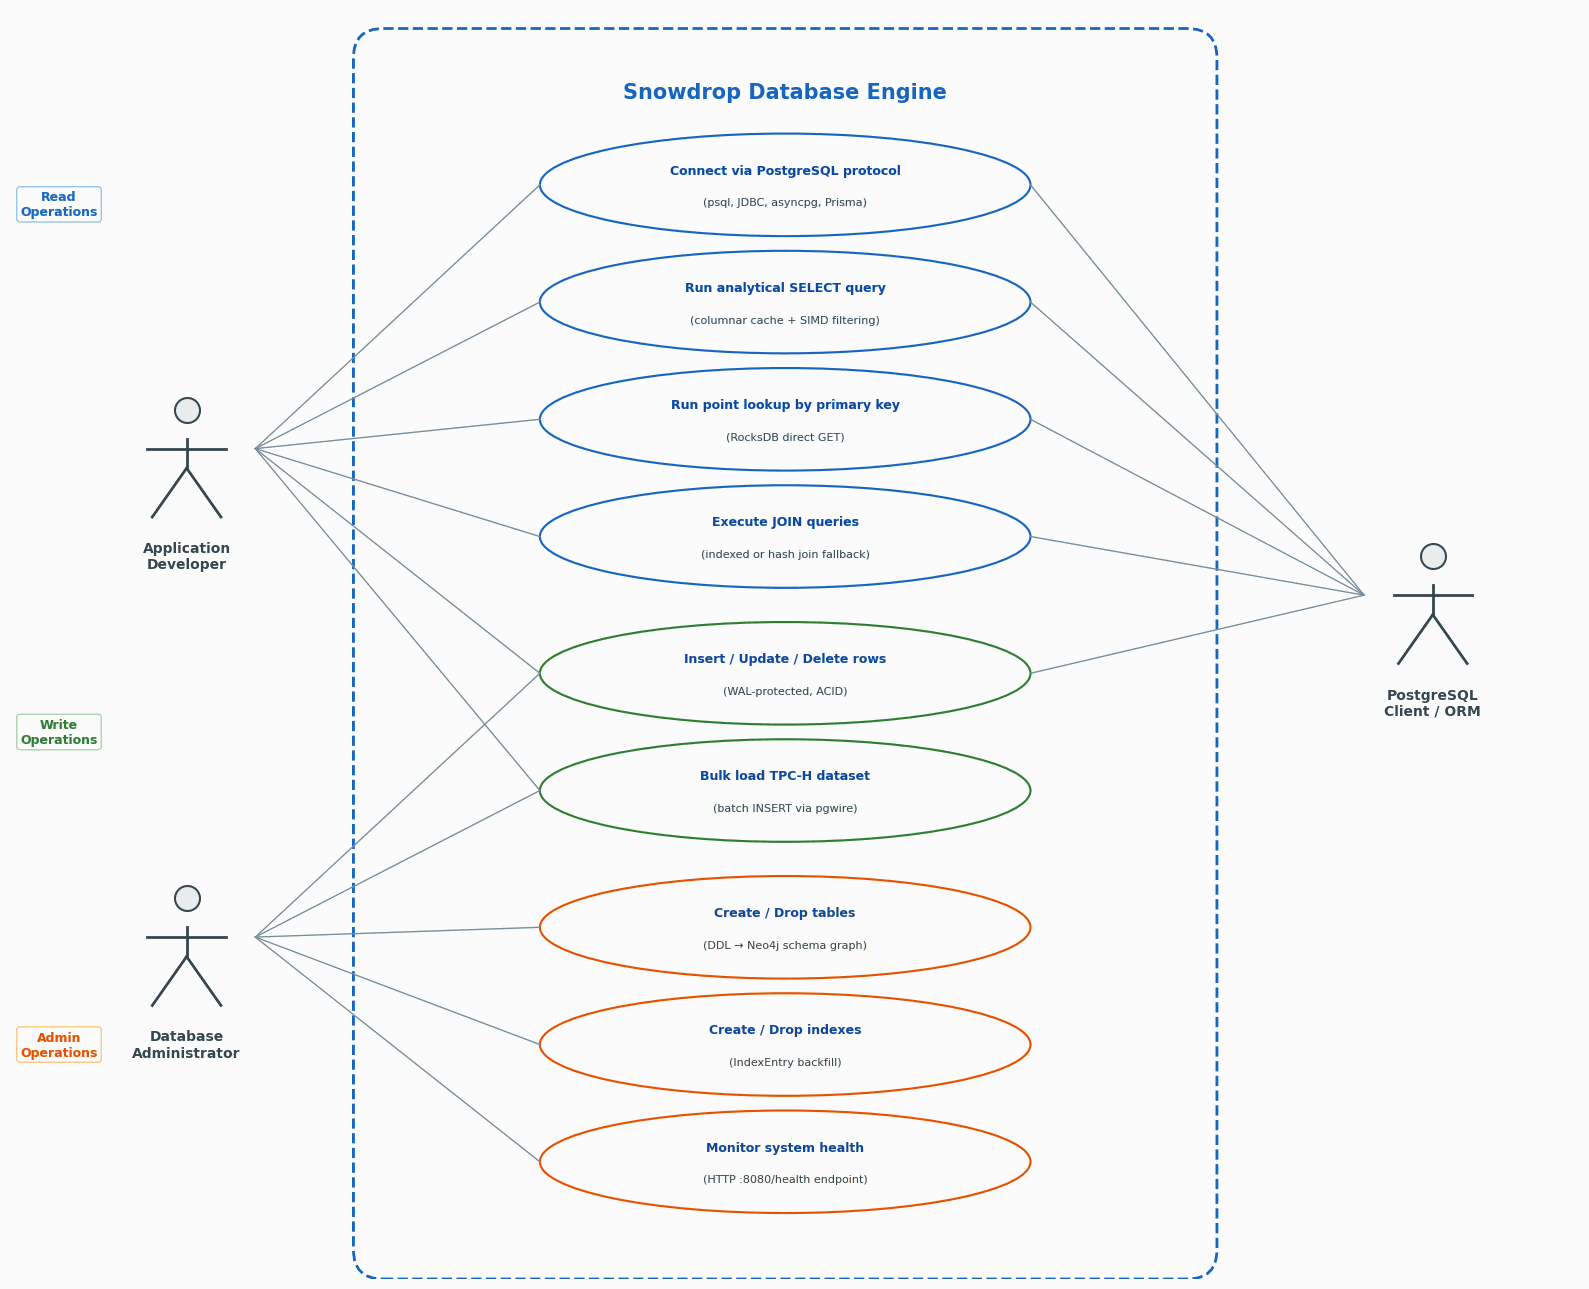
\includegraphics[width=0.95\textwidth]{chapters/chapter05/fig05/02_use_case (1).png}
    \caption{Snowdrop use case diagram}
    \label{fig:usecase}
\end{figure}

The system is designed around three primary actors: application developers, who execute queries and perform write operations; database administrators, who manage schema objects and indexes; and PostgreSQL clients or ORMs, which connect through the standard wire protocol. The use cases are grouped into three categories: read operations, shown in blue; write operations, shown in green; and administrative operations, shown in orange.

\section{Query Execution: SELECT Path}

Figure~\ref{fig:seq-select} presents the execution flow for a \texttt{SELECT} query and the main branching logic inside that process.

\begin{figure}[H]
    \centering
    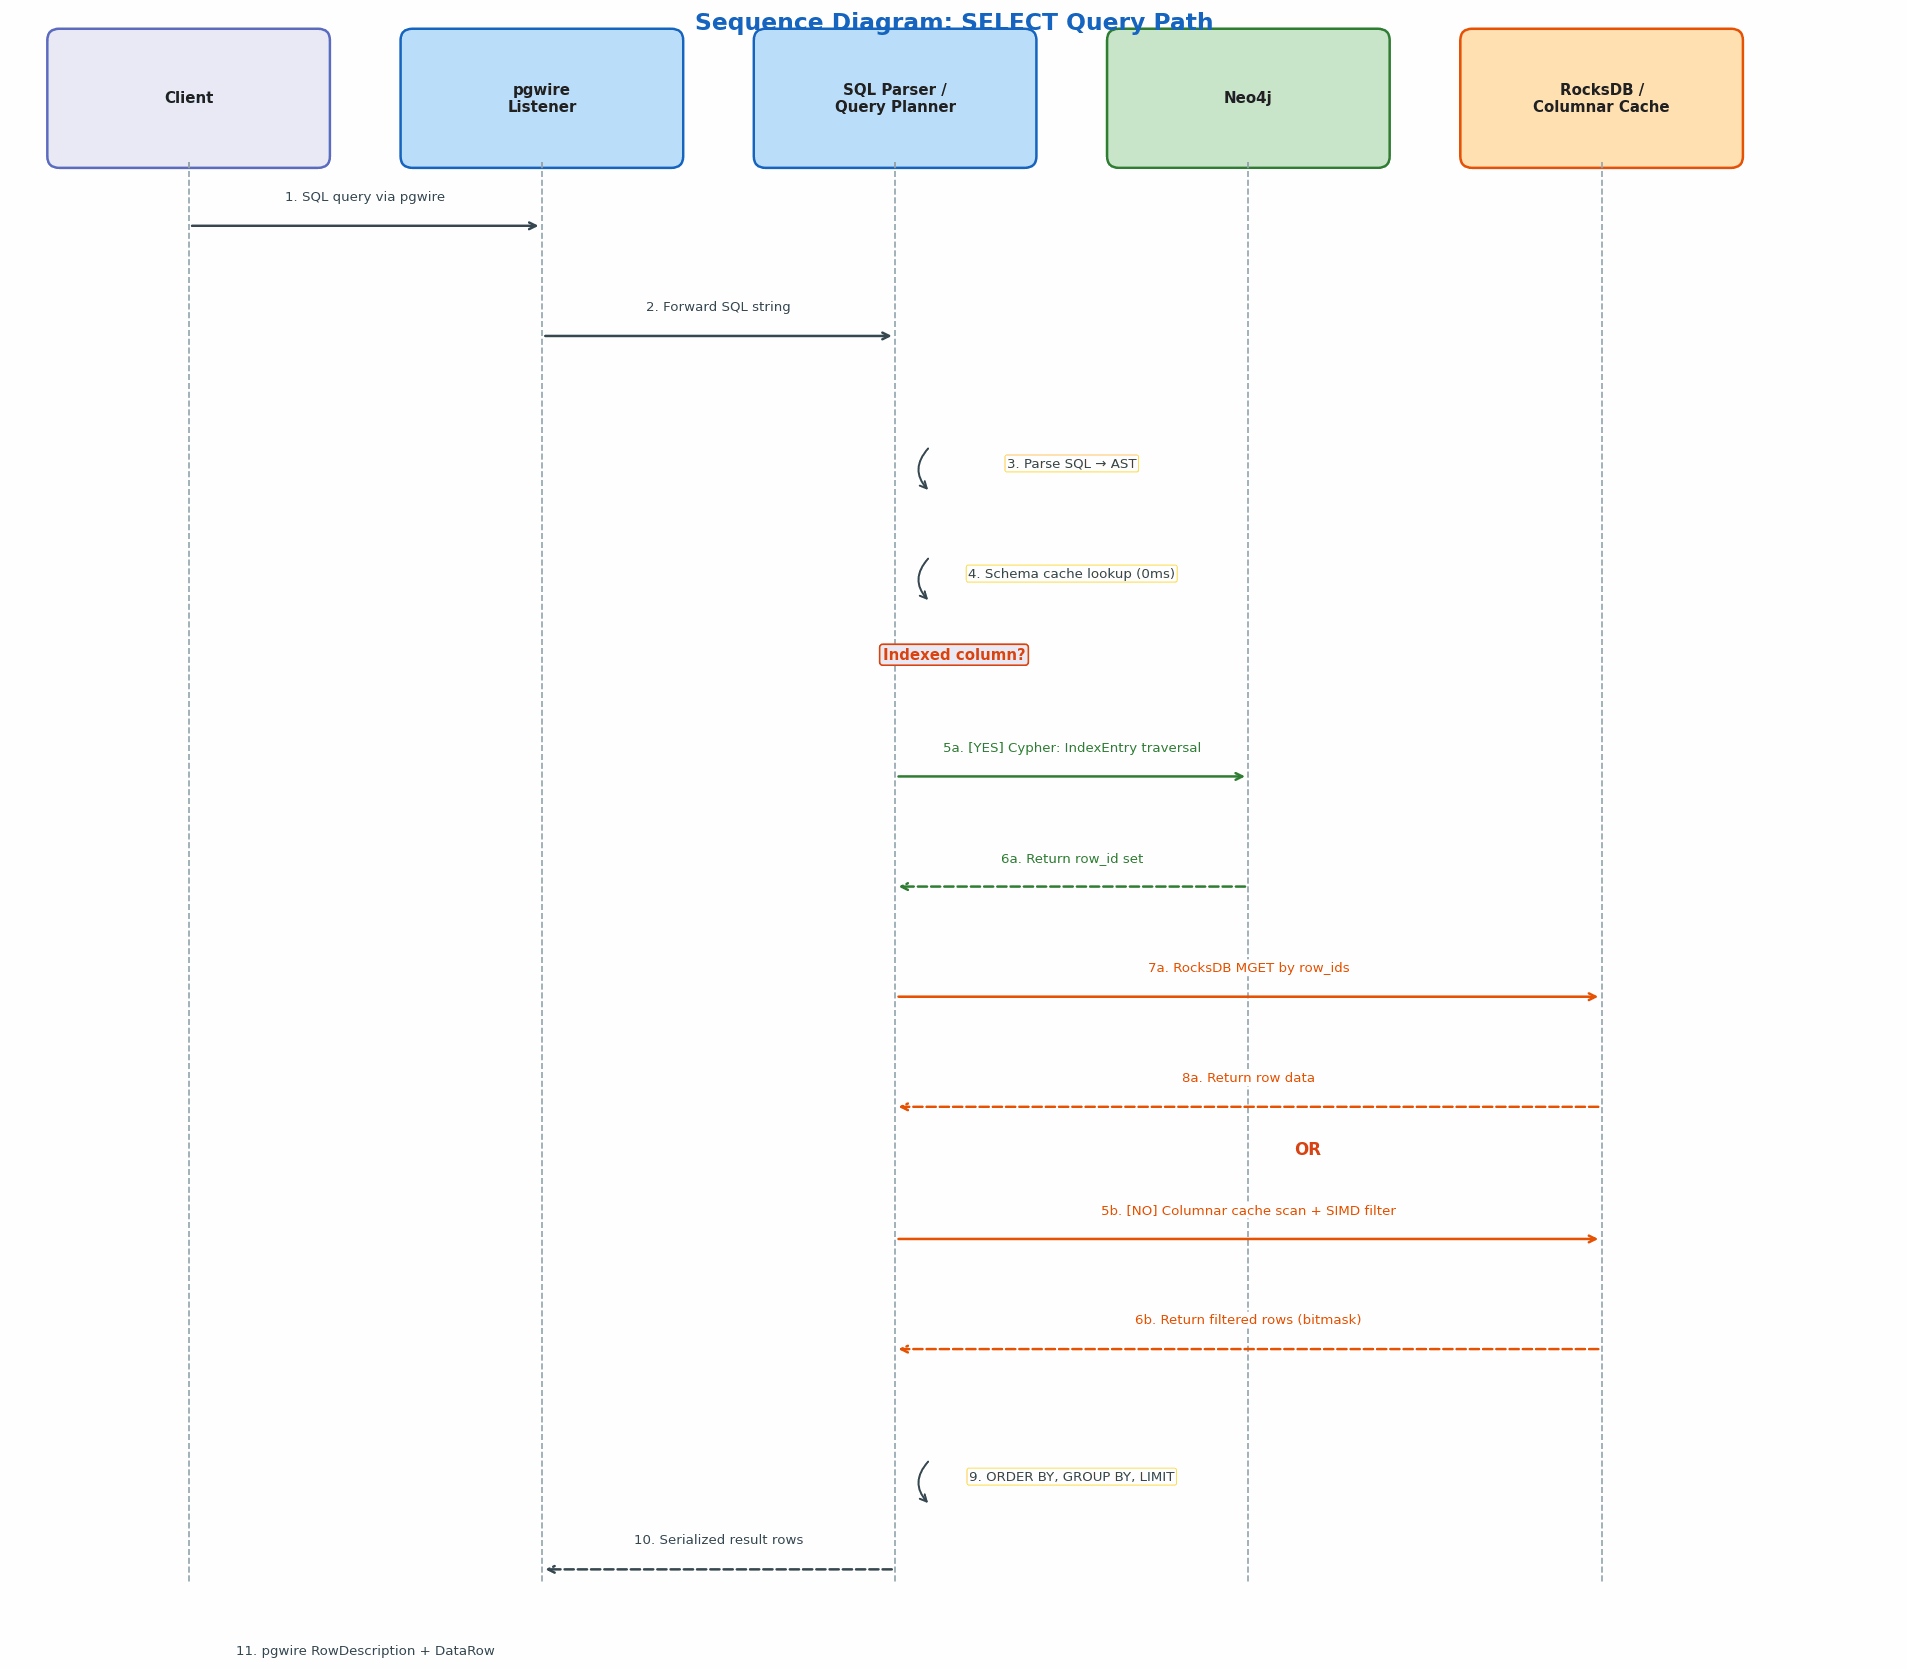
\includegraphics[width=\textwidth]{chapters/chapter05/fig05/03_sequence_select (1).png}
    \caption{Sequence diagram: SELECT query execution path}
    \label{fig:seq-select}
\end{figure}

After the SQL statement is parsed and validated against the schema, execution proceeds along one of several relation-backed paths depending on query shape and available access methods. The \textbf{secondary-index path} uses RocksDB-backed index keys to retrieve the corresponding \texttt{row\_id} values and then performs a batch lookup in RocksDB. The \textbf{columnar path} applies SIMD-accelerated filtering over typed column arrays and produces \texttt{u64} bitmasks that identify matching rows without requiring full tuple deserialization~\cite{zhou2002}. More complex queries --- including joins, subqueries, set operations, and the current practical migration subset --- are routed through a shared relation pipeline in the orchestrator. After that, execution merges at the aggregation and serialization stage, and the results are returned through pgwire.

\section{Write Execution: INSERT Path}

Figure~\ref{fig:seq-insert} shows the \texttt{INSERT} execution path together with the WAL state transitions that protect it.

\begin{figure}[H]
    \centering
    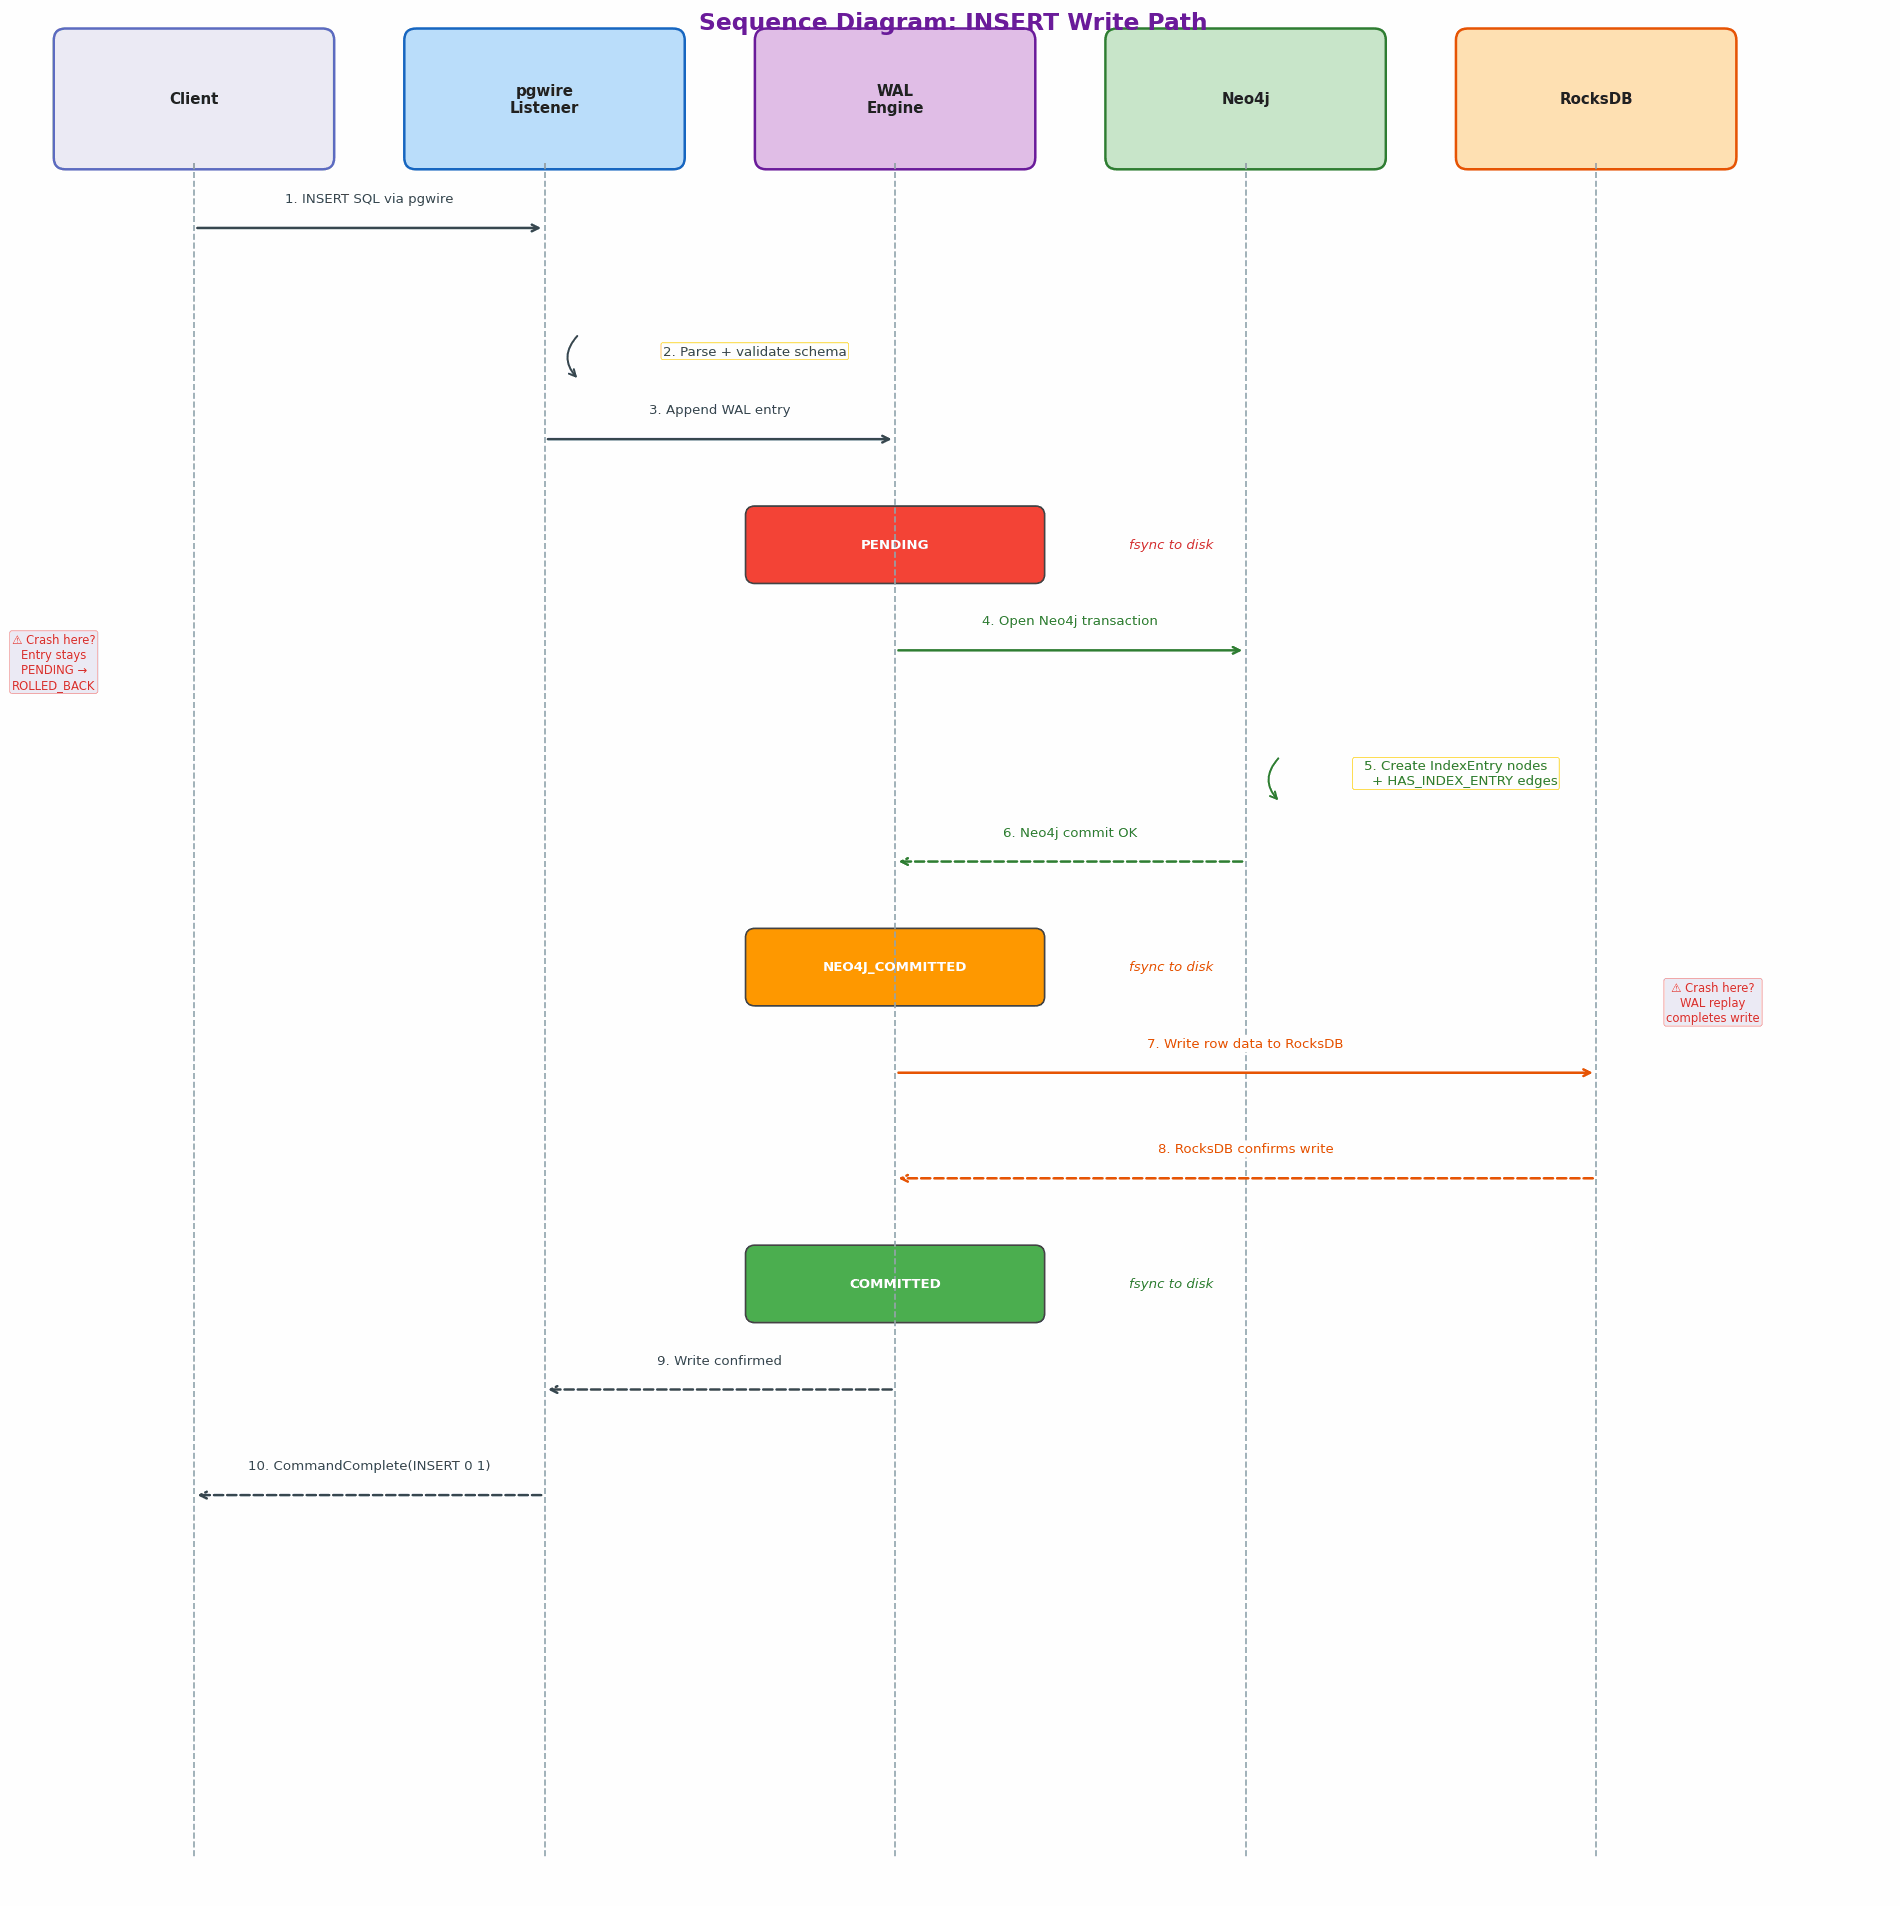
\includegraphics[width=\textwidth]{chapters/chapter05/fig05/04_sequence_insert (1).png}
    \caption{Sequence diagram: INSERT write path with WAL state machine}
    \label{fig:seq-insert}
\end{figure}

Each write operation follows a strictly ordered WAL-protected sequence:
\texttt{PENDING} $\rightarrow$ Neo4j metadata update $\rightarrow$ \texttt{NEO4J\_COMMITTED} $\rightarrow$ RocksDB row/index write $\rightarrow$ \texttt{COMMITTED}$~\cite{mohan1992}$.
Every state transition is flushed to disk using \texttt{fsync}. The diagram also highlights two crash scenarios. If a failure occurs after the Neo4j commit but before the RocksDB write, the WAL is replayed during restart. If the crash happens before the Neo4j commit is completed, the operation is rolled back. This prevents partially completed writes from becoming visible to clients.

\section{Neo4j Metadata Graph}

Figure~\ref{fig:neo4j} presents the Neo4j metadata graph. The original concept included both a schema layer and an index layer, but the current implementation uses Neo4j only for schema metadata while secondary indexes live in RocksDB.

\begin{figure}[H]
    \centering
    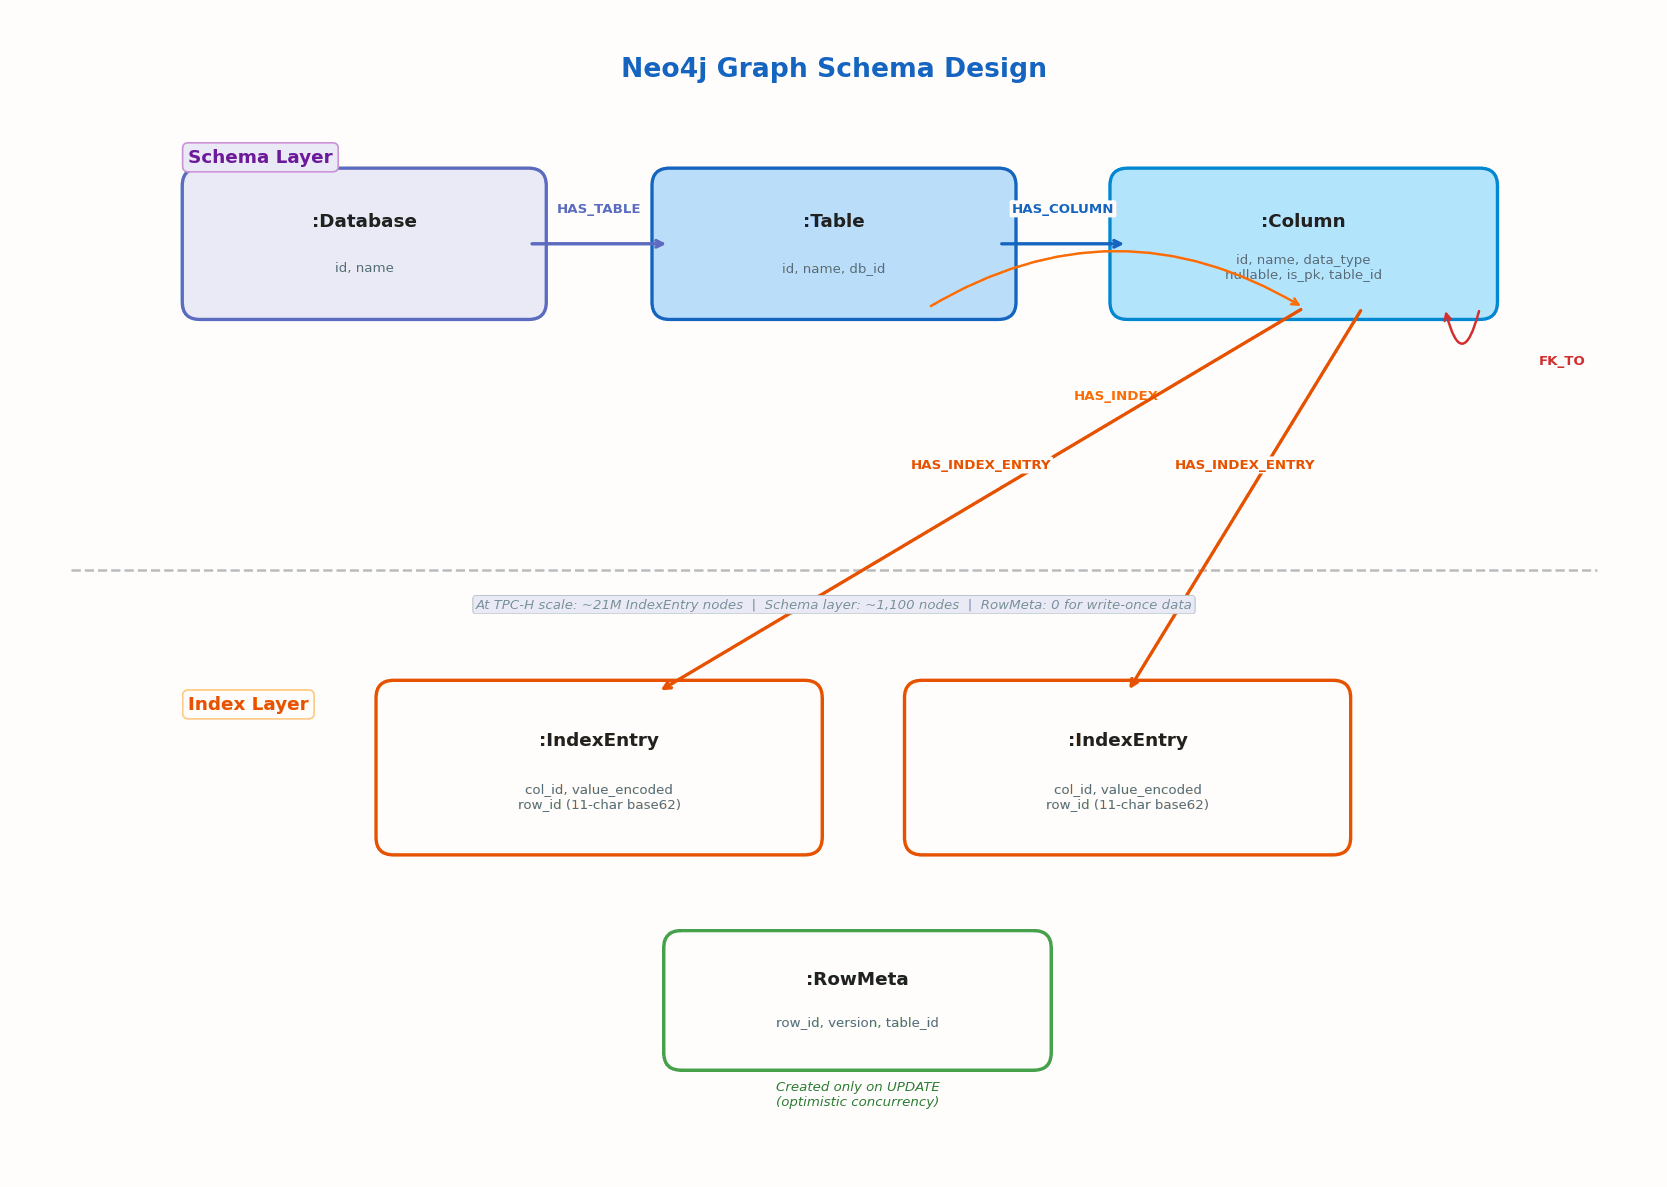
\includegraphics[width=0.95\textwidth]{chapters/chapter05/fig05/05_neo4j_schema (1).png}
    \caption{Neo4j graph schema used for Snowdrop metadata}
    \label{fig:neo4j}
\end{figure}

The metadata graph represents database structure as a directed graph:
\texttt{:Database} $\rightarrow$ \texttt{:Table} $\rightarrow$ \texttt{:Column}, with relationships for foreign keys, constraints, and index metadata. This layer remains relatively small and stable because it grows with schema complexity rather than with row count. In the current implementation, Neo4j is therefore used as the authority for schema description, migration introspection, and constraint-aware planning, while indexed values themselves are stored in RocksDB.

\section{Workspace Structure}

The codebase is organized as a Rust multi-crate workspace consisting of five crates: \texttt{orchestrator} (binary entry point, pgwire listener, relation pipeline, and migration-aware query routing), \texttt{executor} (typed values, DML, filters, and columnar execution), \texttt{wal} (append, replay, and compaction logic), \texttt{schema} (Neo4j operations, DDL, and type validation), and \texttt{keys} (base62 encoding and key construction). These crate boundaries enforce separation of concerns at the compilation level and reduce the risk of accidental cross-module dependencies.
